\documentclass[dvipdfmx]{jsarticle}
\usepackage[dvipdfmx]{graphicx}
\usepackage{amsmath, amssymb}
\usepackage{mathtools}
\usepackage{here}
\begin{document}
\title{週間進捗報告}
\author{権藤陸}
\maketitle
\section{今週の進捗}
\begin{itemize}
    \item いただいたReID論文の読み込み
    \item SRPNetに関連する論文の参照
\end{itemize}

\section{SRPNet}
\subsection{PointNet[1]}
PointNetのClassification Networkをほぼそのまま採用.異なる点は,入力が3 + 1次元となっている部分である.
点群は,以下の3つの重要な性質をもつ.
\begin{itemize}
    \item 順序に依存しない.つまり,N個の3次元点群を処理する場合,データの順序が変わっても,出力は不変であることが望ましい.
    \item 点同士は孤立しているわけではなく,隣接する点が意味のある部分集合を形成している.そのため,モデルは局所構造や局所構造間の相互作用を捉えられる必要がある.
    \item 点群の回転や平行移動といった幾何学変換に対して不変である.
\end{itemize}
基本的には,MLPを重ね,Input transformとFeature transformという層で,アフィン変換を行い,最後にMax Poolingを行う構造になっている.アフィン変換により,回転・移動による不変性を獲得している.また,Max Poolingにより,順序に依存しないモデルとしている.

\subsection{Attention}
4D-PointNetの出力特徴ベクトルを学習して重みを生成し,その重みを出力特徴ベクトルに乗じることで,意味のある特徴を強調している.
SENet[2]と同様の構造だが,全結合層の次元と活性化関数が変更されている.本研究では,Attention Moduleの活性化関数にソフトマックス関数が用いられている.
\subsection{Bi-LSTM}
過去と未来のレーダ点群はどちらも有用で補完し合う関係にあると考えられるため,順方向のLSTMと逆方向のLSTMを組み合わせて使用する.2つのLSTMの出力は,Mean Poolingにより結合される.
\section{classification vs ReID}
論文内で分類タスクとReIDタスクの2つのタスクを行っているが,それら2つのタスクの違いはあまり言及されていない.分類タスクは交差エントロピー誤差を用いて,文字通り分類を行うタスクであるのに対し,ReIDタスクは検索のタスクとみなすことができる.誤差関数には2つの画像の類似度を測るトリプレットロスを用いている.ReIDのテストセットには,ギャラリーとクエリが存在し,与えられたクエリに対し,モデルがギャラリーから最適な候補を順番にk個とってきて,上位k個の中にクエリと同じ人物がいればOkとなる.

Classificationのタスクでは,学習済みの人物だけ識別・分類できればよいが,ReIDではサンプルが少なく学習が十分でない人物についても識別できる必要がある.実用化を考慮すれば,ReIDは識別対象は非協力的な場合が多いため,対象となる人物の人数は多いが,1人あたりのサンプル数は少ないものとなる.また,ReIDではモデルが異なる時間、異なる環境、異なる視点で正確な識別を達成できることが要求される.

\section{損失関数}
\subsection{交差エントロピー誤差}
本研究における交差エントロピー誤差は,ソフトマックス関数との組み合わせで,以下のように記述される.
\begin{equation}
    L_{cls} = -\frac{1}{N}\sum_{b=1}^{N} \sum_{b=1}^{K} y_{ub} \cdot \log{(\frac{e^{Z ub}}{\sum_{v=1}^{K} e^{Z vb}})}
\end{equation}

ここで、$u$と$v$は出力が属するカテゴリ、$K$はカテゴリの総数、$N$はバッチ内のサンプルの総数、$y_ub$はサンプル$b$に対するカテゴリ$u$のラベルである.これに正則化項を追加し,分類タスクで用いる損失関数となる.
\begin{equation}
    L = L_{cls} + \omega \cdot L_{reg} = L_{cls} + \omega \cdot ||I - AA^T||_{F}^2
\end{equation}

ここで、$L_{cls}$は分類損失、$L_{reg}$は正則化項損失、$I$は単位行列、$A$は特徴変換行列、$\omega$は重みで、0.001に設定されている。
\subsection{トリプレットロス}
\begin{equation}
    L_{triplet} = \max{(d_p - d_n + \alpha, 0)}
\end{equation}

$d_p$と$d_n$はそれぞれ同一人物からの特徴量と異なる人物からの特徴量の$L_2$距離である。$\alpha$はトリプレットロスのマージンである。トリプレットロスにより、同一人物からの特徴量は近くなり、異なる人物からの特徴量は遠くなる。
\section{結果}
\begin{itemize}
    \item classificationの精度
    \item 
SRPNet-15モデルでは,15人の個人に対して平均98.16\% の精度を達成.SRPNet-40モデルでは,40人の個人に対して平均91.50\% の精度を達成.
    \item ReIDのCMC, mAP

\begin{figure}[htbp]
\begin{center}
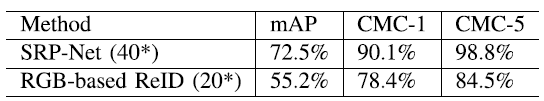
\includegraphics[width=0.8\linewidth]{./img/ReID_result.png}
\end{center}
\caption{ReIDタスクの結果}
\end{figure}
\end{itemize}
\begin{figure}[htbp]
\begin{center}
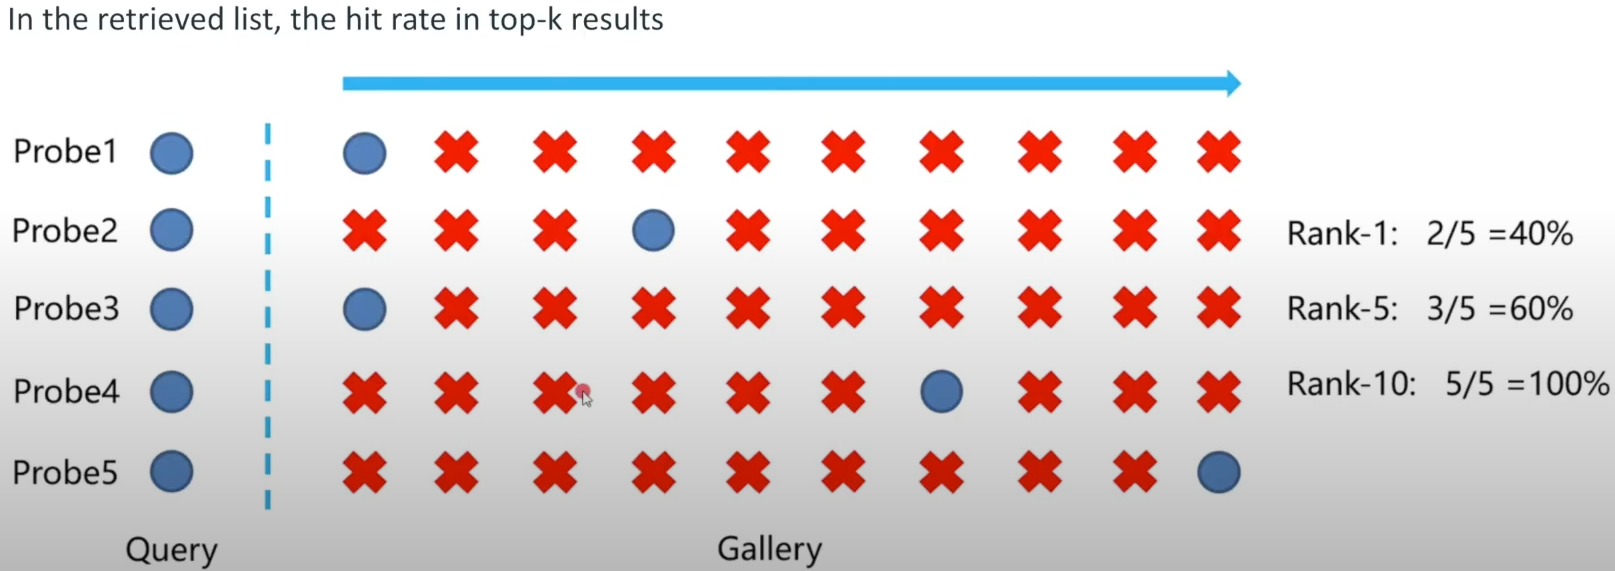
\includegraphics[width=0.8\linewidth]{./img/cmc.png}
\end{center}
\caption{CMCの計算の模式図[3]}
\end{figure}

\begin{figure}[htbp]
\begin{center}
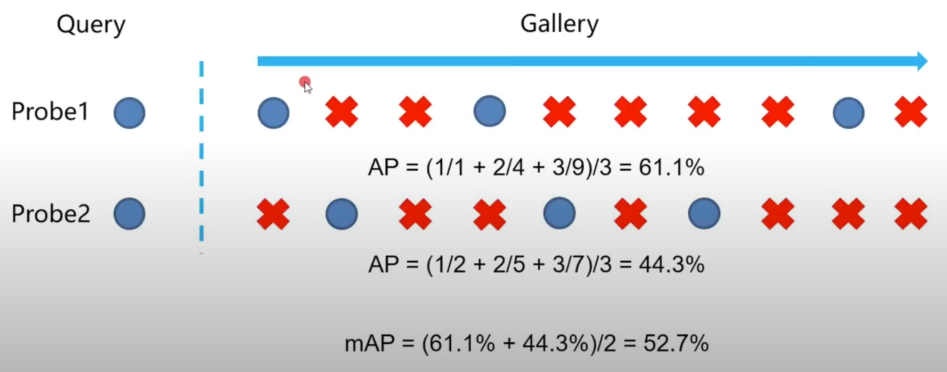
\includegraphics[width=0.8\linewidth]{./img/mAP.png}
\end{center}
\caption{mAPの計算の模式図[3]}
\end{figure}

\section{計画}
\begin{itemize}
    \item ReID論文の読み込み
    \item スライド作成
\end{itemize}
\begin{thebibliography}{}
\bibitem [1] Qi, Charles R., et al. "Pointnet: Deep learning on point sets for 3d classification and segmentation." \textit{Proceedings of the IEEE conference on computer vision and pattern recognition}. 2017.
\bibitem [2] Hu, Jie, Li Shen, and Gang Sun. "Squeeze-and-excitation networks." \textit{Proceedings of the IEEE conference on computer vision and pattern recognition}. 2018.
\bibitem [3] DDeep Person Re-identification Introduction, https://www.youtube.com/watch?v=BPNQqHpLSGk
\end{thebibliography}
\end{document}